\section{Results and Conclusion}
The implementation with automatic differentiation from ngsolve is not extremely complicated but not as straight forward as one would hope for. A big problem with this approach are the different types of objects in ngsolve, namely \obj{float}, \obj{CoefficientFunction}, \obj{Parameter} and \obj{SumOfIntegrals}, which are not easy to concatenate the right way to achieve the desirable function.
This does not occur for the stokes equation or shape function, but complex side constraints are tougher than necessary.

The \fun{DiffShape()} function helps to eliminate the need to derive and transform the terms in the Lagrangian ourselves, but is e.g. not usable for \obj{VectorH1} functions. 
With the automatic Differentiation we were able to achieve the desired form:
The volume constraint is very important for this piece and is possible to be implemented with and or without differentiation. This was also showed in a programming example, that this term on its own can deform any shape to the desired volume.
On the other hand, the barycenter constraint does not hold up to its expectations. None of our implemented terms does give the desired functionality and others we are not able to implement in ngsolve.

Even without the barycenter constraint we were able to achieve this solution after 300 iterations:

% figure olive

The derived shape derivative of the paper \cite{nearly_conformal_paper} does not show the same behavior as the one created from \fun{DiffShape()}. That means we were also not able to create a solution that looks similar to the one before.

\begin{figure}
\begin{minipage}{.5\textwidth}
    \centering
    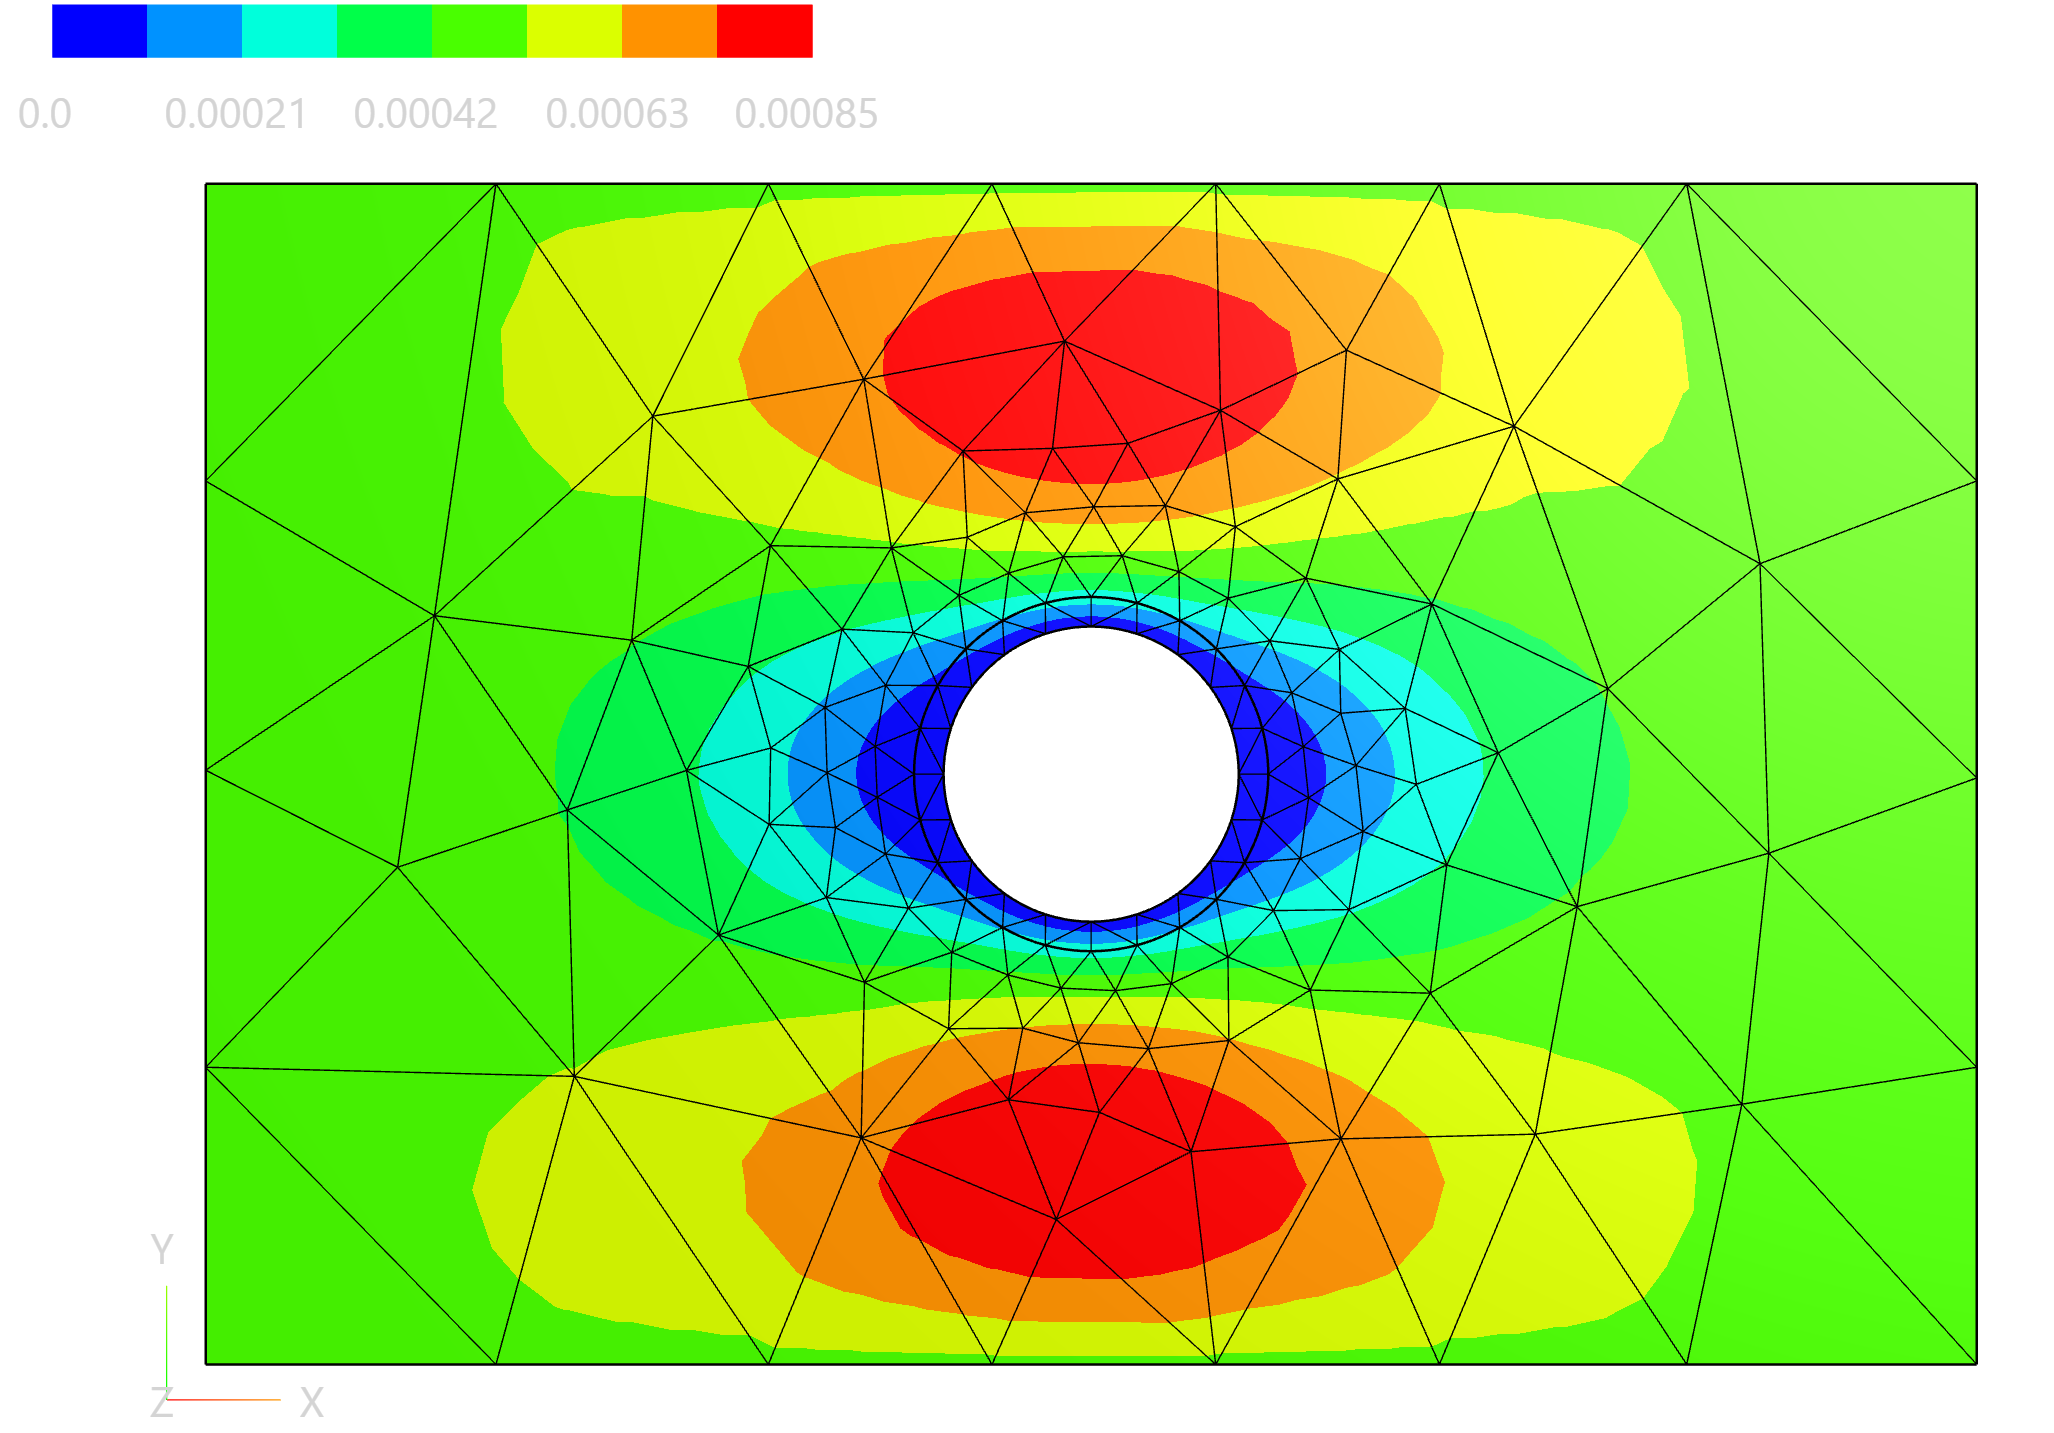
\includegraphics[width=1\textwidth]{figures/u_0.PNG}
    \caption{ $\mathbf{||u||_2}$ on $\Omega_{\mathrm{n}}$ for $\mathrm{n}=0$}
    \label{plot_ref_u_0}
\end{minipage}
\begin{minipage}{.5\textwidth}
    \centering
    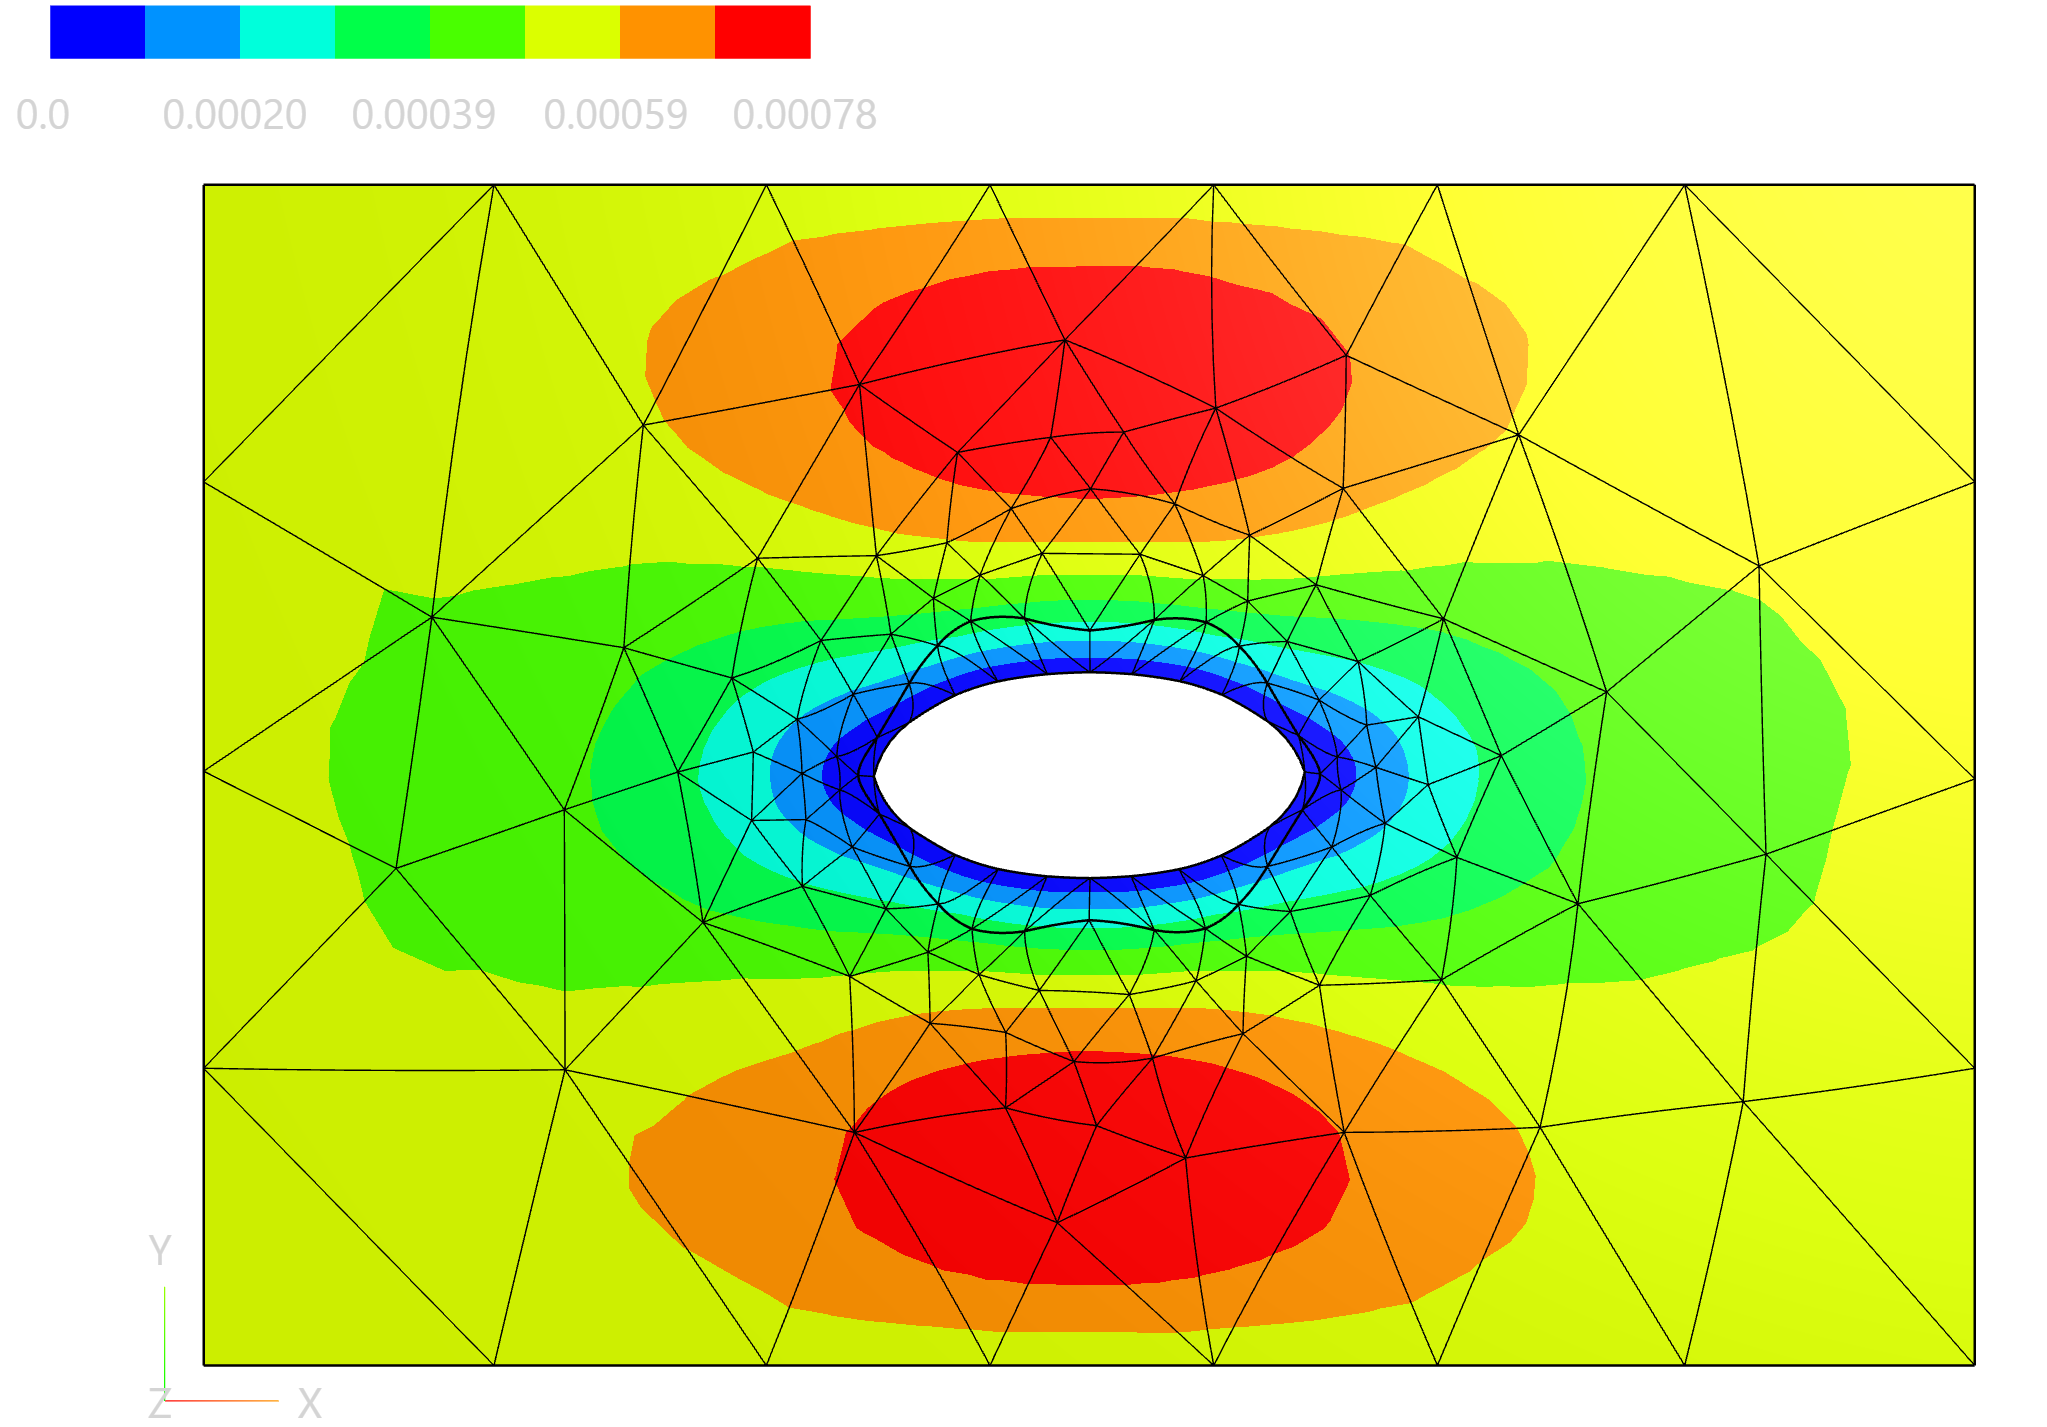
\includegraphics[width=1\textwidth]{figures/u_final.PNG}
    \caption{ $\mathbf{||u||_2}$ on $\Omega_{\mathrm{n}}$ for $\mathrm{n}=800$}
    \label{plot_ref_u_final}
\end{minipage}
\end{figure}

\begin{figure}
    \begin{center}
        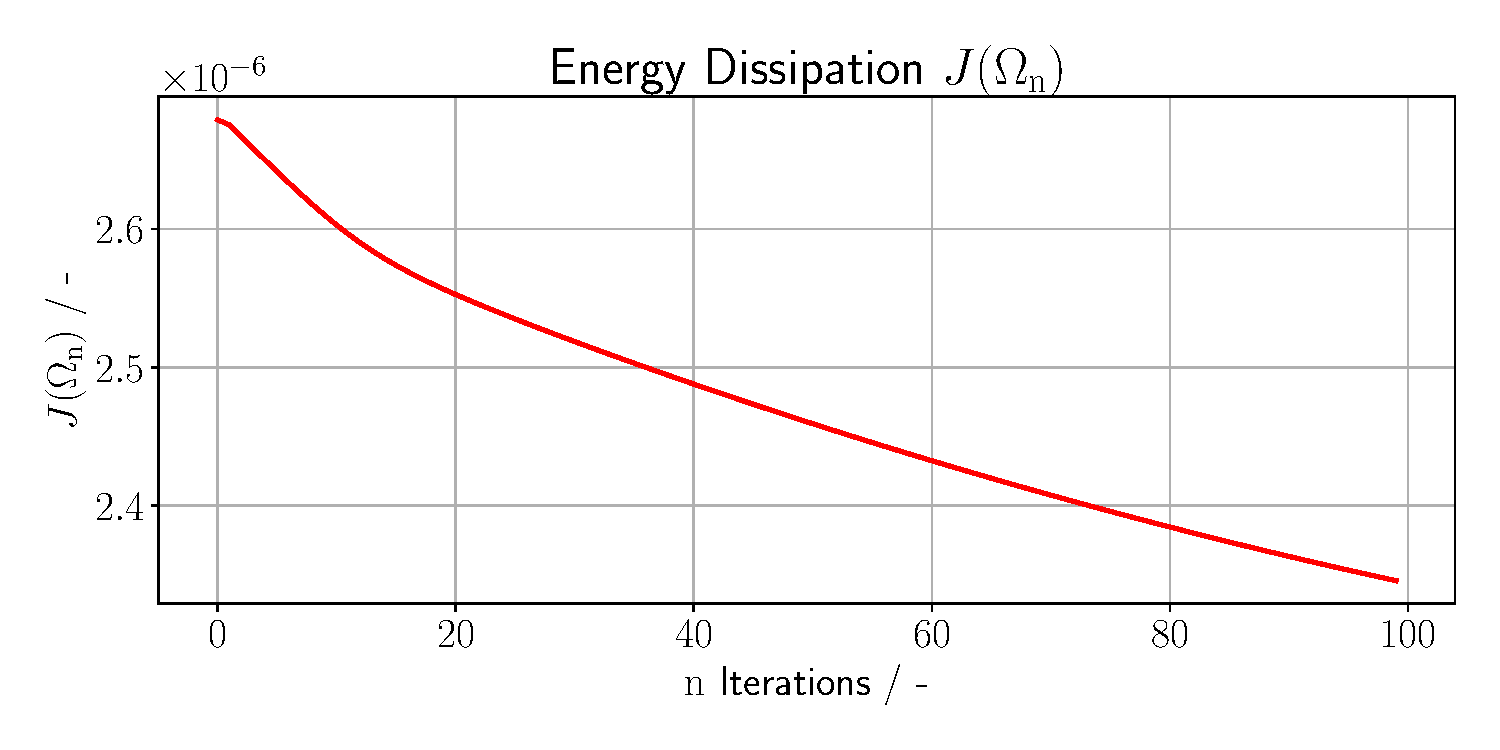
\includegraphics[width=0.95\textwidth]{figures/energy_diss_plot.pdf}
        \caption{Evaluation of Energy Dissipation on $\Omega$}
        \label{plot_ref_energy_diss}
    \end{center}
\end{figure}

\begin{figure}
    \begin{minipage}{.5\textwidth}
        \centering
        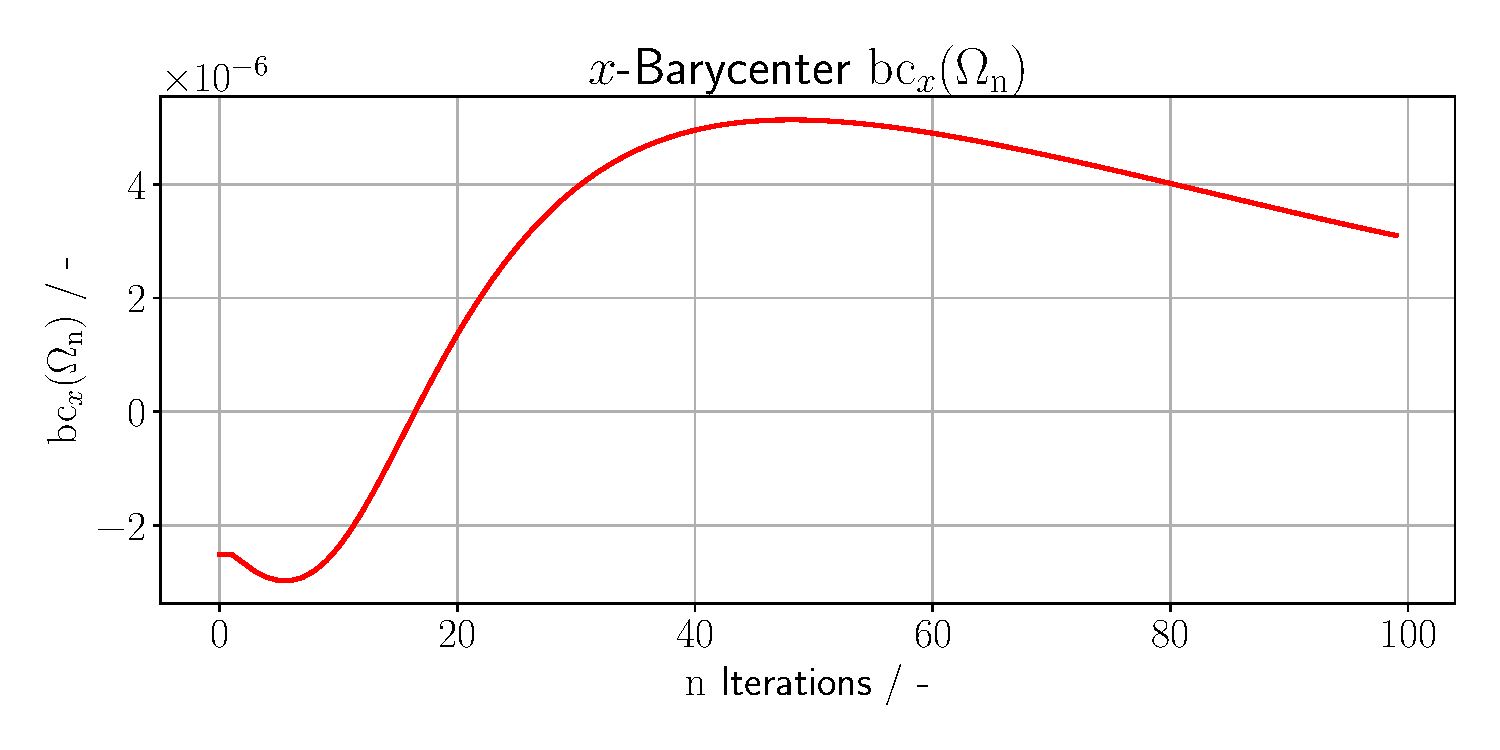
\includegraphics[width=1\textwidth]{figures/bc_x__plot.pdf}
        \caption{$x$ Component of Barycenter of $\Omega$}
        \label{plot_ref_bc_x}
    \end{minipage}
    \begin{minipage}{.5\textwidth}
        \centering
        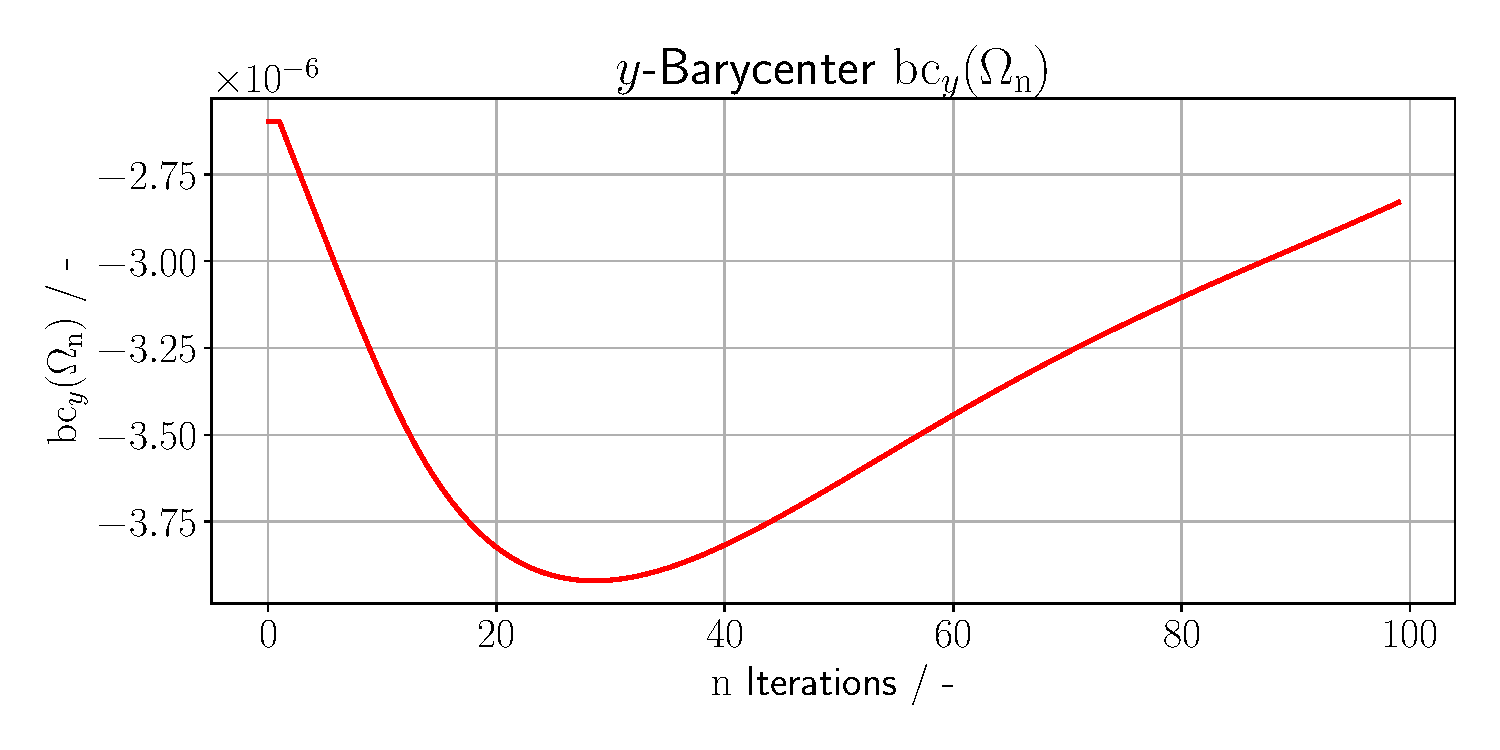
\includegraphics[width=1\textwidth]{figures/bc_y_plot.pdf}
        \caption{$y$ Component of Barycenter of $\Omega$}
        \label{plot_ref_bc_y}
    \end{minipage}
    \end{figure}

\begin{figure}
    \begin{center}
        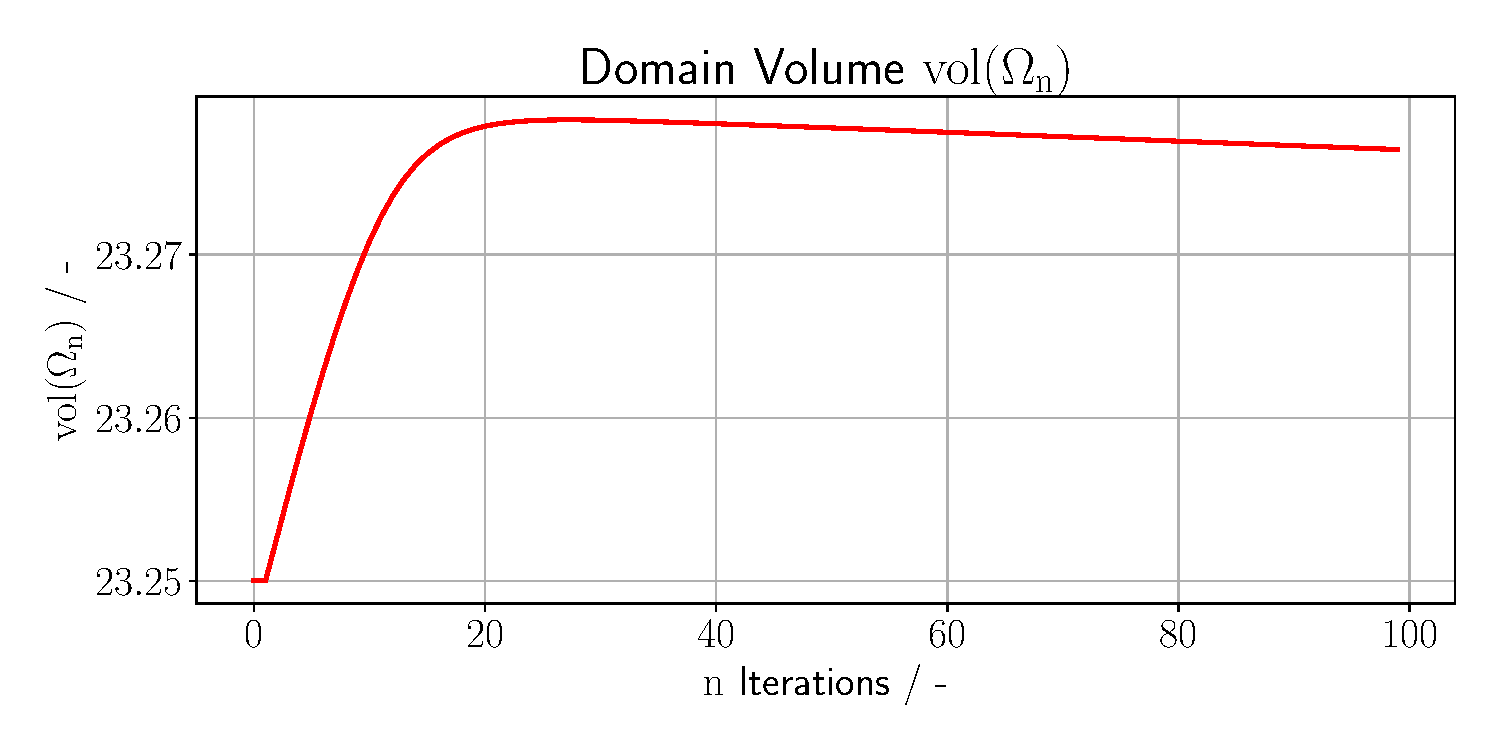
\includegraphics[width=0.95\textwidth]{figures/volume_plot.pdf}
        \caption{Volume of $\Omega$}
        \label{plot_ref_volume}
    \end{center}
\end{figure}

\begin{figure}
    \begin{minipage}{.5\textwidth}
        \centering
        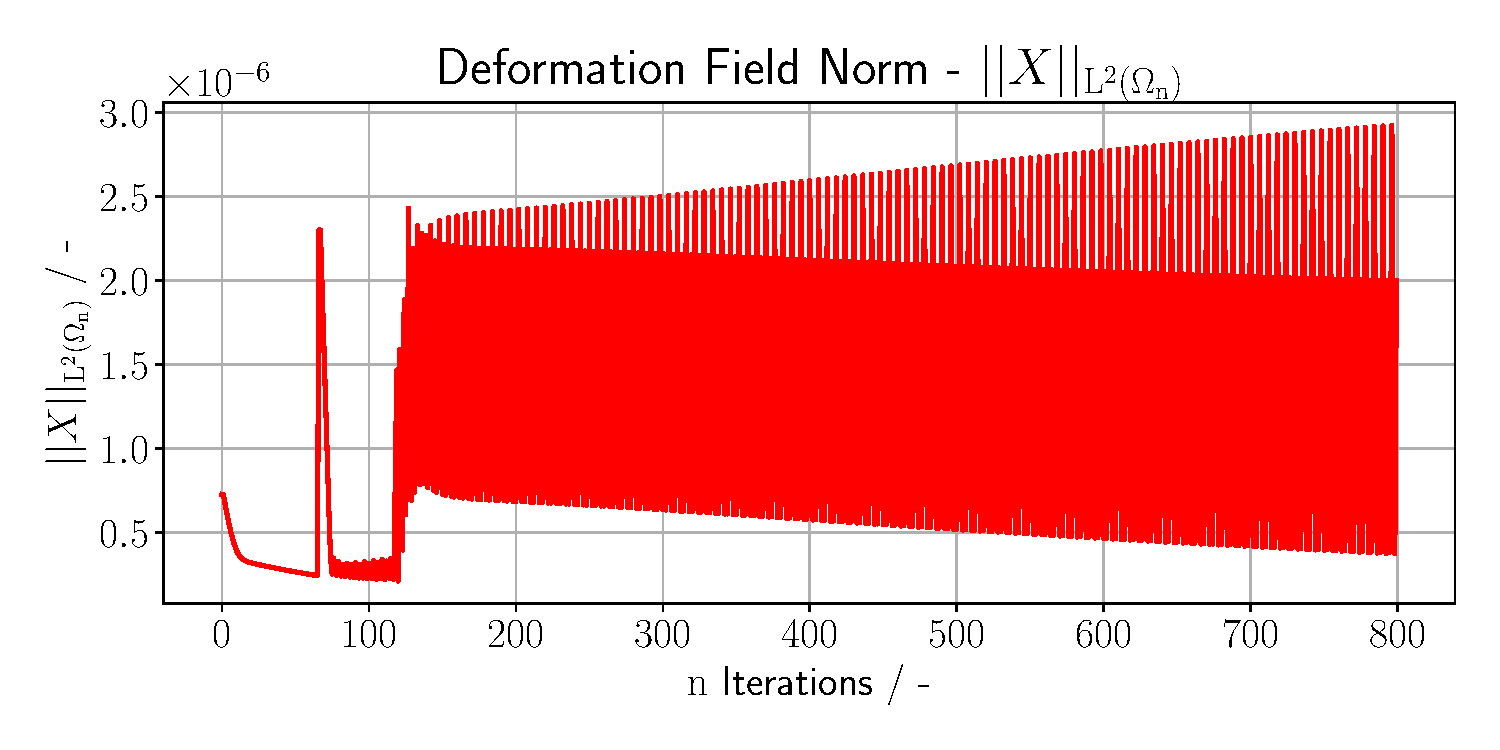
\includegraphics[width=1\textwidth]{figures/gfxnorm_plot.pdf}
        \caption{Norm of $X$ on Domain}
        \label{plot_ref_norm}
    \end{minipage}
    \begin{minipage}{.5\textwidth}
        \centering
        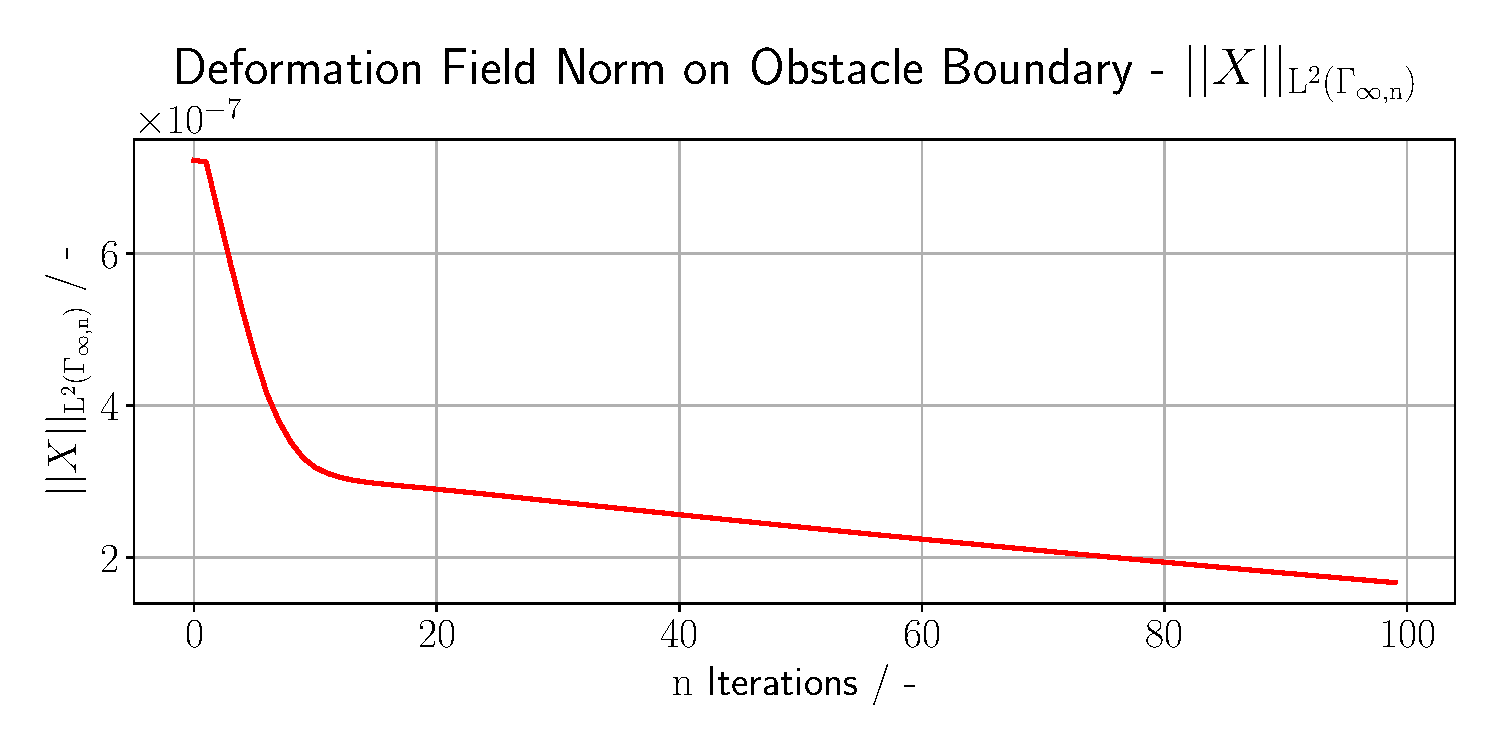
\includegraphics[width=1\textwidth]{figures/gfx_bndnorm_plot.pdf}
        \caption{Norm of $X$ on Boundary}
        \label{plot_ref_bndnorm}
    \end{minipage}
    \end{figure}